\label{sec:hardsoft}
Our hardware-software co-design DSLAM system contains two essential improvements in the pose estimation and the place recognition tasks. As illustrate in \cref{fig:all_us}, both of these two components are divide into two stages: 1) CNN front end to extact features which is deployed to the CNN acclerator on PL and 2) geometric operations to present final results which is depoyed on the PS ARM core. To make full use of the Zynq MPSoC (illustrated in \cref{fig:plps}), we optimize the data follow for both of these components.

\subsection{Pose Estimation}
We adopt Depth-VO-Feat \cite{Zhan:2018e92} in DSLAM system to estimate the pose from the input monocular camera. Monocular visual SLAM is a key issue in the field of robotics, while there are two challenging problems: 1) it's difficult and expensive to obtain accurate labeled data. 2) the methods that use monocular sequences in training always suffer from the scale-ambiguity problem, i.e. the actual scale of translations is missing and only direction is learned. In Depth-VO-Feat \cite{Zhan:2018e92}, we use image reconstruction loss as a self-supervised signal to train the convolutional neural networks, and jointly train two networks for depth and odometry estimation without external supervision, which can be used independently in testing phase. Besides, to fix scale-ambiguity issue, we use stereo sequences in training phase and monocular sequences in testing phase. With the known spatial relationship between the left and right cameras, our neural networks can learn the real world scale. Feature reconstrution loss is an additional supervision signal, used to improve the robustness of this framework. And we use depth smoothness loss to encourage the predicted depth to be smooth, which demonstrated success in prior works. Then the final loss becomes $$L=\lambda_{ir}L_{ir}+\lambda_{fr}L_{fr}+\lambda_{ds}L_{ds}$$, where $L_{ir}$, $L_{fr}$ and $L_{ds}$ are image reconstruction loss, feature reconstruction loss and depth smoothness loss respectively, $\lambda_{ir}$, $\lambda_{fr}$ and $\lambda_{ds}$ are the loss weightings for each loss term. The training framework is illustrated in \cref{fig:dvo}.

\begin{figure}[thb]  
    \centering  
    {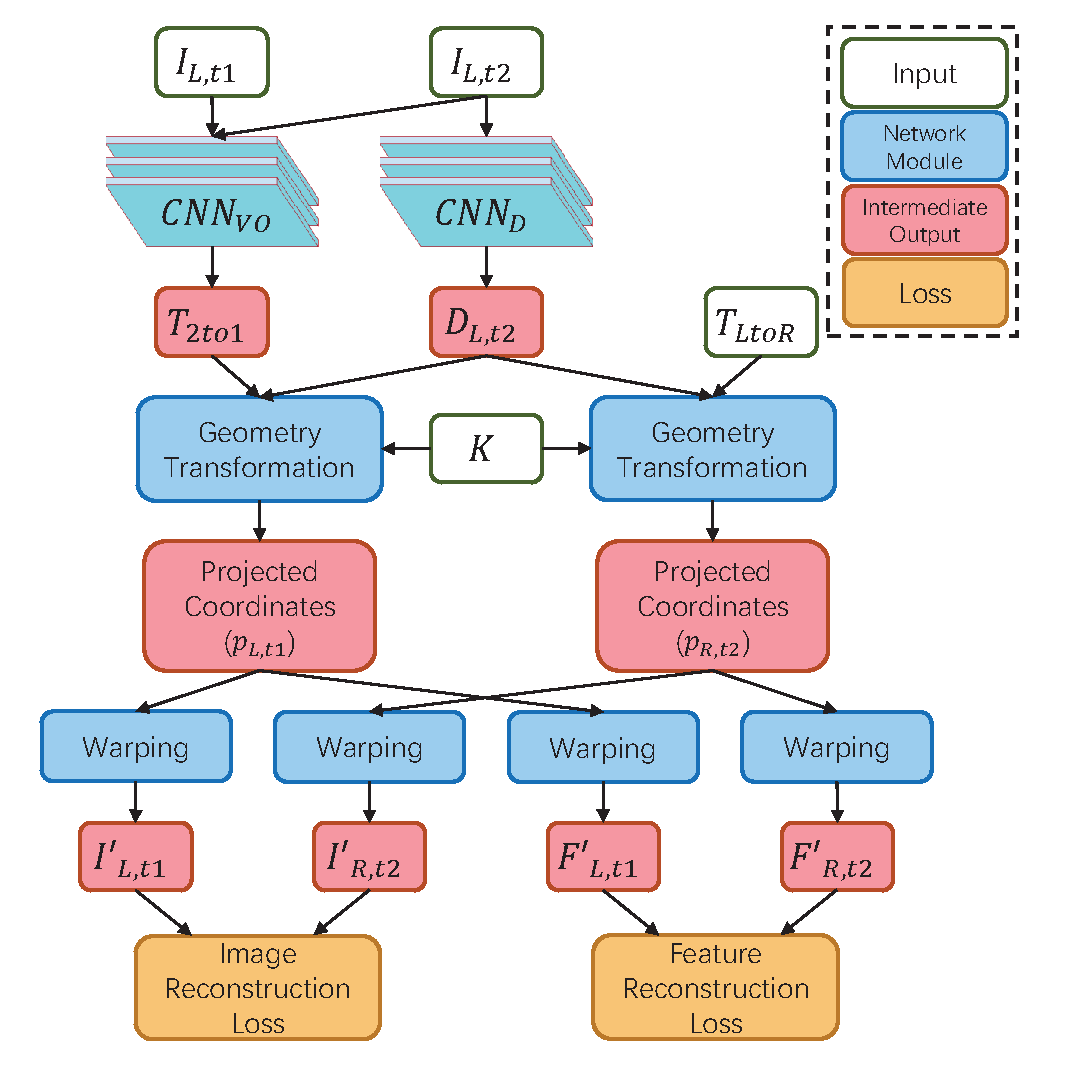
\includegraphics[width=0.95\linewidth]{fig/depth_vo_feat.eps}\label{fig:dvo}}
    \caption{Illustration of Depth-VO-Feat framework in training phase, where $T_LtoR$ is the relative camera pose transformations between right and left views, and $K$ denotes the known camera intrinsic matrix. $CNN_{VO}$ and $CNN_D$ can be used independently in testing phase. }
\end{figure}

In order to run efficiently on the FPGA platform, we use fixed-point arithmetic units in the hardware to replace the floating-point number format in GPU and CPU. Many previous works have shown that 8-bit quantization for weights and featuremaps can make the networks run faster on FGPA. Here we adopt the fixed-point finetune method in \cite{Yu:2018:IDC:3299999.3283452}, in that we use the fixed-point number representation in the feed forward phase and keep floating-point number representation for backpropagation, and both weights and data will be re-quantized after each backpropagation. As the fixed-point method can leads to the accuracy loss of the model, We attempt several different quantization strategies to balance speed and accuracy, which will be shown in detail in \cref{sec:experiment}.

\subsection{Place Recognition}
As described in \cref{sec:background}, CNN has achieved great improvements in place recognition tasks. 
